\documentclass{article}
\usepackage[UTF8]{ctex}  % 中文支持
\usepackage{graphicx}    % 插图
\usepackage{hyperref}    % 超链接
\usepackage{listings}    % 代码块
\usepackage{amsmath}     % 数学
\usepackage{caption}     % 图标题
\usepackage{geometry}    % 页面设置
\geometry{margin=1in}

\title{中期作业报告}
\author{李孟霖 2311067}
\date{}

\begin{document}

\maketitle

\section{规约求和实现概述}

在这个规约求和的实现中,首先将输入数组按 block 求和,返回每个 block 的规约求和结果构成的数组,然后在 CPU 端使用 C++ 的 \texttt{numeric} 库进行最终的求和。整个过程将使用 CUDA 事件来测量时间。

相关的核函数及其声明写在 \texttt{kernels.cu} 和 \texttt{kernels.cuh} 中。

\subsection{第一版规约求和}

这个版本中,设备端求和完全使用全局内存。下面是运行截图和 ncu 分析结果。

\begin{figure}[h]
    \centering
    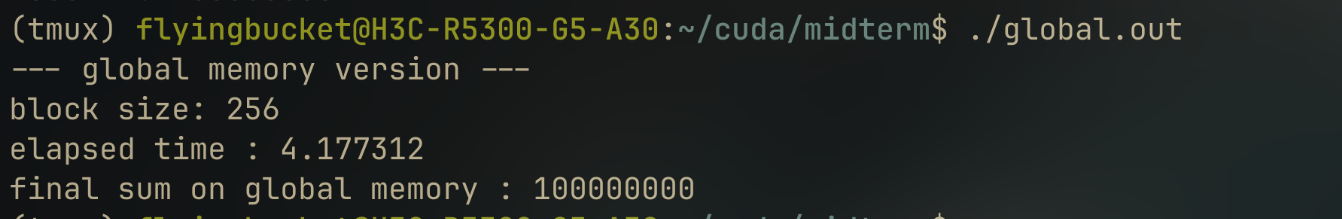
\includegraphics[width=0.7\linewidth]{./images/reduce_v1.png}
    \caption{第一版规约求和运行截图}
\end{figure}

% \begin{figure}[h]
%     \centering
%     \includegraphics[width=0.7\linewidth]{./images/reduce_v1_ncu.png}
%     \caption{第一版规约求和 ncu 分析结果}
% \end{figure}

考虑使用共享内存来进行初步优化,使用 shuffle 指令来进一步加速 block 内的规约求和。

\subsection{第二版规约求和}

在第二版中,使用共享内存来进行 block 内的规约求和。每个 block 的线程将数据加载到共享内存中,但暂不使用 shuffle 指令。下面是运行截图和 ncu 分析结果。

\begin{figure}[h]
    \centering
    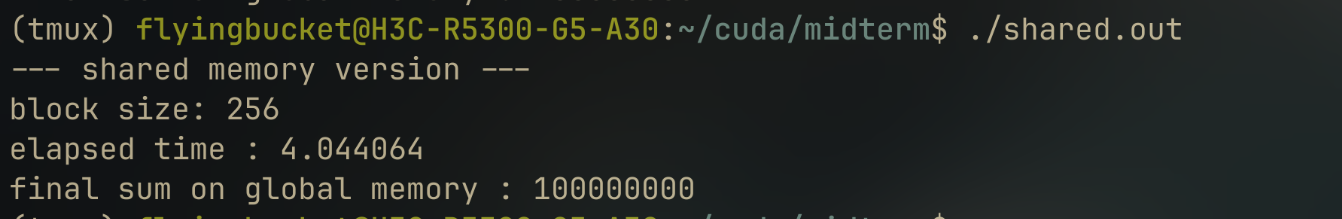
\includegraphics[width=0.7\linewidth]{./images/reduce_v2.png}
    \caption{第二版规约求和运行截图}
\end{figure}

% \begin{figure}[h]
%     \centering
%     \includegraphics[width=0.7\linewidth]{./images/reduce_v2_ncu.png}
%     \caption{第二版规约求和 ncu 分析结果}
% \end{figure}

% \subsection{第三版规约求和}

在第三版中,使用了 shuffle 指令来进一步加速 block 内的规约求和。每个 block 的线程将数据加载到共享内存中,并使用 shuffle 指令进行规约求和。下面是运行截图和 ncu 分析结果。

\begin{figure}[h]
    \centering
    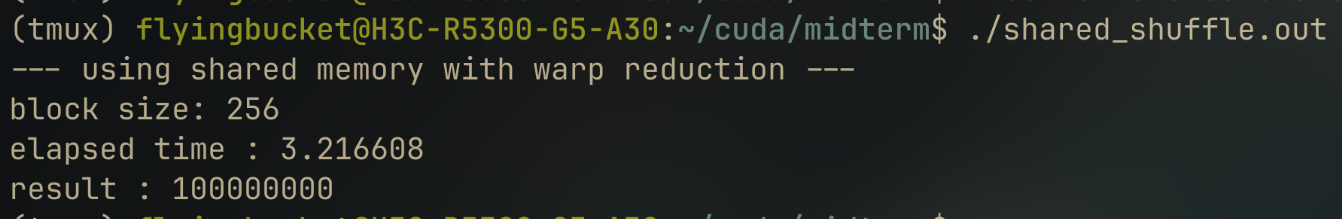
\includegraphics[width=0.7\linewidth]{./images/reduce_v3.png}
    \caption{第三版规约求和运行截图}
\end{figure}

% \begin{figure}[h]
%     \centering
%     \includegraphics[width=0.7\linewidth]{./images/reduce_v3_ncu.png}
%     \caption{第三版规约求和 ncu 分析结果}
% \end{figure}

\section{总结}

通过这三个版本的实现,我们可以看到使用共享内存和 shuffle 指令对规约求和的性能有显著提升。每一版相较上一版在运行时间上都有大约 10\% 到 25\% 的提升。

\end{document}
